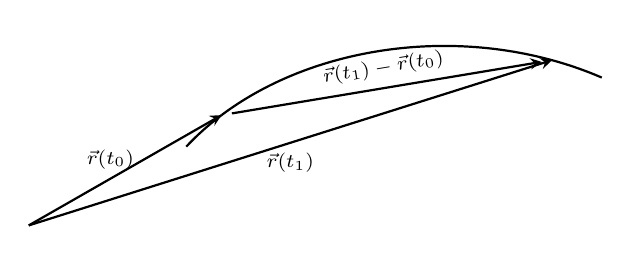
\begin{tikzpicture}[>=stealth]
	

\draw [thick,{\colorone}] (2,1) arc [x radius=4,y radius=3,start angle=145,end angle=135] node (A) {};
\draw [thick,{\colorone}] (A.center) arc [x radius=4,y radius=3,start angle=135,end angle=70] node (B) {};
\draw [thick,{\colorone}] (B.center) arc [x radius=4,y radius=3,start angle=70,end angle=60];



\draw [thick,->] (0,0) -- (A.center) node [left,pos=.6] {\scriptsize $\vec r(t_0)$};
\draw [thick,->] (0,0) -- (B.center) node [below,pos=.5] {\scriptsize $\vec r(t_1)$};
\draw [->,thick,{\colortwo}] (A)--(B) node [above,black,pos=.5,sloped] {\scriptsize $\vec r(t_1)-\vec r(t_0)$};
\end{tikzpicture}

